\documentclass{article}
\usepackage{tikz}

\pgfkeys{/tikz/.cd,%
  circle height/.initial=0,     %initial value
  circle height/.get=\circleheight, %to get the value from a macro
  circle height/.store in=\circleheight, %to store the value into a macro
  diameter/.initial=1,
  diameter/.get=\diameter,
  diameter/.store in=\diameter,
  circle color/.initial=red,
  circle color/.get=\circlecolor,
  circle color/.store in=\circlecolor,
}

\newcommand{\pgfdoublecircle}[1][]{%
  \tikzset{circle color=red,diameter=1,#1} %the default options will be overwritten by the one introduced
  \fill[\circlecolor](0,\circleheight) circle (\diameter/2);
  \fill[\circlecolor](\diameter/2,\circleheight) circle (\diameter/2);
}

\begin{document}
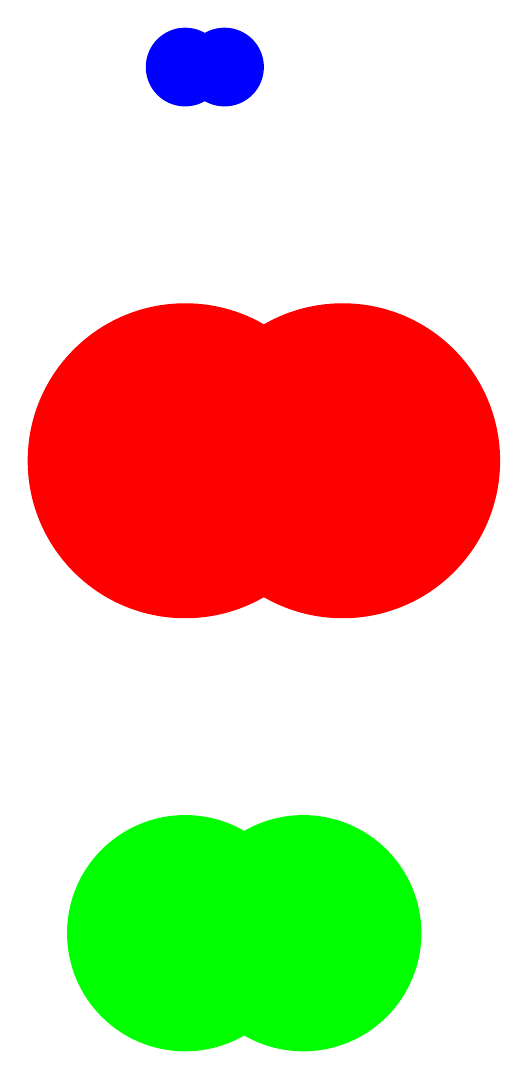
\begin{tikzpicture}[y=-1cm]
\pgfdoublecircle[circle color=blue]
\pgfdoublecircle[circle height=5,diameter=4]
\pgfdoublecircle[circle height=11,diameter=3,circle color=green]
\end{tikzpicture}

\end{document}